\documentclass[11pt]{article}
\usepackage{amsmath,amssymb, amsthm, marvosym, permute, extsizes}
\usepackage{graphicx, float, enumitem, adjustbox, hyperref, bm}
\usepackage{microtype, dsfont}
\usepackage[separate-uncertainty = true]{siunitx}
\usepackage[normalem]{ulem}
\usepackage{braket}
\usepackage[T1]{fontenc}
\usepackage[utf8]{inputenc}
\usepackage{lmodern}
\usepackage{mhchem}
\usepackage{gensymb}
\usepackage[T1]{fontenc}
\usepackage[a4paper,margin=2.5cm]{geometry}
\usepackage[icelandic]{babel}
\usepackage{tikz}
\newcommand{\explain}[2]{\underbrace{#1}_\textrm{$#2$}}
\usepackage{minted}
\usemintedstyle{perldoc}
\parindent = 0pt
\usepackage{fancyhdr}
    \pagestyle{fancy}
    \headheight=32pt
    \lhead{Háskóli Íslands\\Raunvísindadeild}
    \rhead{Verkleg Eðlisfræði}
\title{{\Huge Leiðniskömmtun}}
\author{Emil Gauti Friðriksson og Garðar Árni Skarphéðinsson}
\date{Apríl 2019 \\
\vspace{5cm}

\includegraphics[width = .6\textwidth]{HIlogo1.png}}

\begin{document}

\maketitle
\thispagestyle{empty}

\newpage

\section{Inngangur}
Þessi tilraun gengur út á það að ná fram skömmtun á leiðni rafstraums með myndun nanóvíra. Leitað er að þessum skammtafræðilegu áhrifum í þrem vírum úr mismunandi efnum, gulli, kopar og platínu/iridíum blöndu. 

\section{Líkan}
Ímyndum okkur rafstraum $I$ sem rennur um nanóvír. Lýsa má þessum straum sem $I = e/\tau$, það er að segja, sem flæði rafeinda á einhverjum tíma $\tau$. Orka rafeindar í vírunum er einfaldlega $E = V e$, þar sem $V$ er spennan yfir vírinn. Nýtum okkur nú óvissulögmál Heisenbergs, en það segir okkur að $\Delta E\Delta t \geq h/2\pi$. Gerum ráð fyrir að óvissan í orku rafeindarinnar sé af stærðargráðunni $\sim E$ og að óvissan í tíma sé af stærðargráðunni $\sim \tau$, en þá fæst

\begin{align}
\Delta E \Delta t \sim E \tau = (Ve)\left( \frac{e}{I} \right) \sim h
\end{align}

En nú er leiðni þessa vírs $G = 1/R = I/V$, þannig að við endum með 

\begin{align}
G \sim \frac{e^2}{h}
\end{align}

Að lokum skulum við margfalda með $2$ til þess að taka spunastefnu rafeindanna til greina, og bæta við heiltölumargfaldaranum $n$ þar sem rafstraumur berst aðeins með heiltölufjölda rafeinda. Við endum þá með skilgreiningu okkar á grunnskammti leiðninnar

\begin{align}
G_n = n \frac{2e^2}{h}, \qquad  n \in \{1, 2, 3 ...\}
\label{eq:leidni}
\end{align}

Þessi skömmtum leiðninar leiðir til skömmtunar rafstraums. Einnig kemur inn í jöfnu~(\ref{eq:leidni}) dreifistuðull, $0<T\leq 1$, en í úrvinnslu gerum við ráð fyrir $T=1$. Ef nanóvír tengir rafrás sem hefur viðnám $R_0$ og spenna $V_0$ er sett á rásina fæst straumurinn

\begin{align}
I_n = \frac{V_0}{R_{TOT}} = \frac{V_0}{R_0 + \frac{1}{G_n}} = \frac{V_0}{R_0 + \frac{h}{2e^2 n}} = \frac{V_0 / R_0}{1 + \frac{h}{2e^2 R_0 n}}
\end{align}

En af þessari jöfnu sjáum við að þegar $n$ stefnir á $+\infty$ þá stefnir straumurinn $I_n$ einfaldlega á $I_0 = V_0 / R_0$.

\section{Framkvæmd og Úrvinnsla}
Tilraunin byggist á myndun nanóvíra á milli tveggja, lítilla makróskópískra víra. Þegar tveimur þannig vírum er slegið saman mynda þeir snertu sem leiðir rafstraum á milli þeirra. Þegar þeir togast aftur í sundur minnkar snertiflötur þeirra þó atómin í vírunum toga samt hvert í annað. Við þetta myndast oft einn nanóvír eða jafnvel fleiri. Þetta var gert við vírana sem minnst var á hér að ofan, sem allir eru mismjúkir, og var fylgjst grannt með straumnum í þeim með hjálp sveiflusjár. Vírarnir voru tengdir við spennugjafa og $\SI{1}{k \ohm}$ viðnám.
\begin{figure}[H]
    \centering
    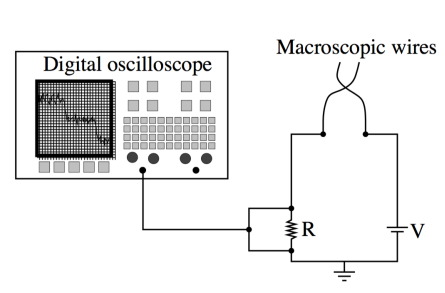
\includegraphics[width=0.4\textwidth]{leidni_skyring.PNG}
    \caption{Uppstilling}
    \label{fig:uppstilling}
\end{figure}

\subsection{Gull}
%V_0 = 0.1011, 50 micrometers
Tveir gullvírar af þykkt $\SI{50}{\mu m}$ eru tengdir við rásina og spennan yfir viðnámið mældist sem $\SI{0.1011}{V}$. Vírarnir eru látnir titra þannig að endi annars þeirra sláist í hinn og myndi tengi á milli þeirra í örskamman tíma. Fylgst er með rafstrauminum á sveiflusjánni og mæld gildi hans eru skráð niður. 

\begin{figure}[H]
    \centering
    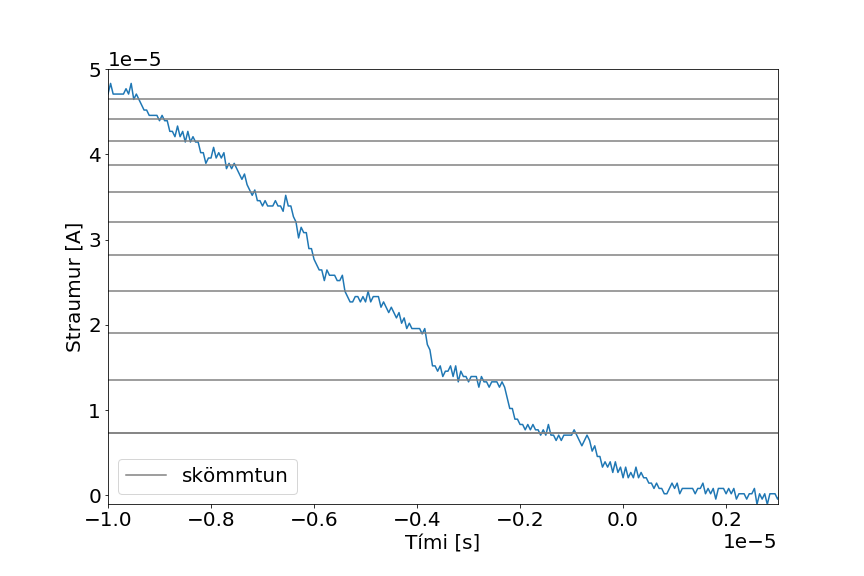
\includegraphics[width=0.8\textwidth]{gull-straumur.png}
    \caption{Straumur í gullvírunum sem fall af tíma. Láréttu línurnar tákna skömmtuðu gildi straumsins sem búist er við miðað við líkanið.}
    \label{fig:gull_straumur}
\end{figure}

Af mynd~\ref{fig:gull_straumur} sjáum við greinileg þrep í staumnum sem svara til fyrstu þriggja skömmtunargildanna, en eftir það verður erfiðara að greina áhrifin. 

\begin{figure}[H]
    \centering
    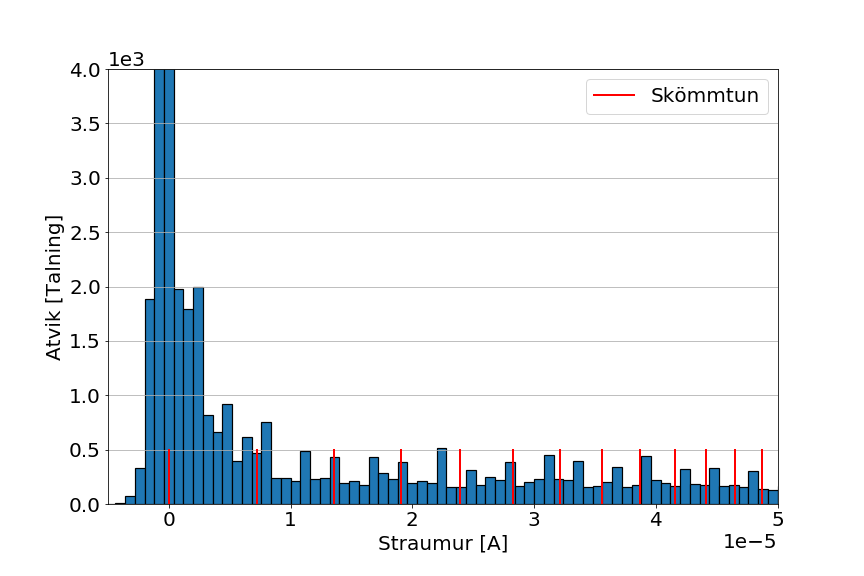
\includegraphics[width=0.8\textwidth]{gull-hist-straumur.png}
    \caption{Tíðnirit fyrir mæld gildi straums í gullvírunum. Rauðu lóðréttu línurnar tákna skömmtuðu gildi straumsins sem búist er við miðað við líkanið.} 
    \label{fig:gull_hist_straumur}
\end{figure}

Á mynd~\ref{fig:gull_hist_straumur} sjáum við greinilega toppa við fyrsta skammtaða gildið, og þar á eftir sjást litlir toppar hér og þar sem sumir falla að líkaninu á meðan aðrir virðast aðeins hliðraðir. \\
Nú má nota gildi spennunar til þess að þessi gögn sýni leiðni frekar en straum.

\begin{figure}[H]
    \centering
    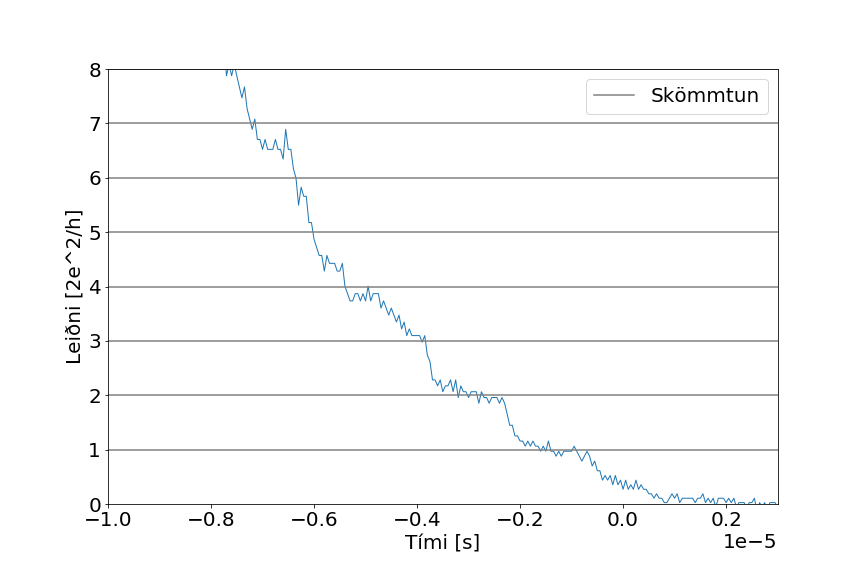
\includegraphics[width=0.8\textwidth]{gull-leidni.png}
    \caption{Leiðni í gullvírunum sem fall af tíma. Láréttu línurnar tákna skömmtuðu gildi leiðninnar sem búist er við miðað við líkanið.}
    \label{fig:gull_leidni}
\end{figure}

Aftur virðast nú vera skýr þrep fyrir fyrstu tvö skömmtuðu gildin á mynd~\ref{fig:gull_hist_leidni} en þar fyrir ofan er erfitt að greina skömmtun. 

\begin{figure}[H]
    \centering
    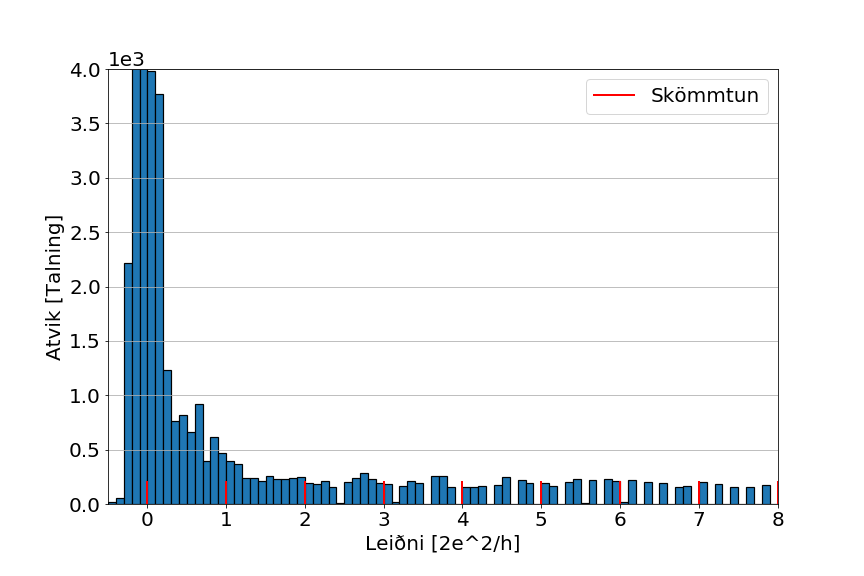
\includegraphics[width=0.8\textwidth]{gull-hist-leidni.png}
    \caption{Tíðnirit fyrir mæld gildi leiðninnar í gullvírunum. Rauðu lóðréttu línurnar tákna skömmtuðu gildi sem búist er við miðað við líkanið.} 
    \label{fig:gull_hist_leidni}
\end{figure}

Við sjáum hér á mynd~\ref{fig:gull_hist_leidni} aftur móta fyrir skýrum topp fyrir fyrsta skammtaða gildið en þaðan af þyrfti líklega fleiri mælingar til þess að eitthvað marktækt væri greinilegt. 


\subsection{Kopar}
%V_0 = 0.1025, 0.5 mm, 99.98% puuure
Nú var gullvírunum skipt út fyrir $\SI{0.5}{mm}$ þykka koparvíra. Spennan mældist nú sem $\SI{0.1025}{V}$ og sömu mælingar voru framkvæmdar.

\begin{figure}[H]
    \centering
    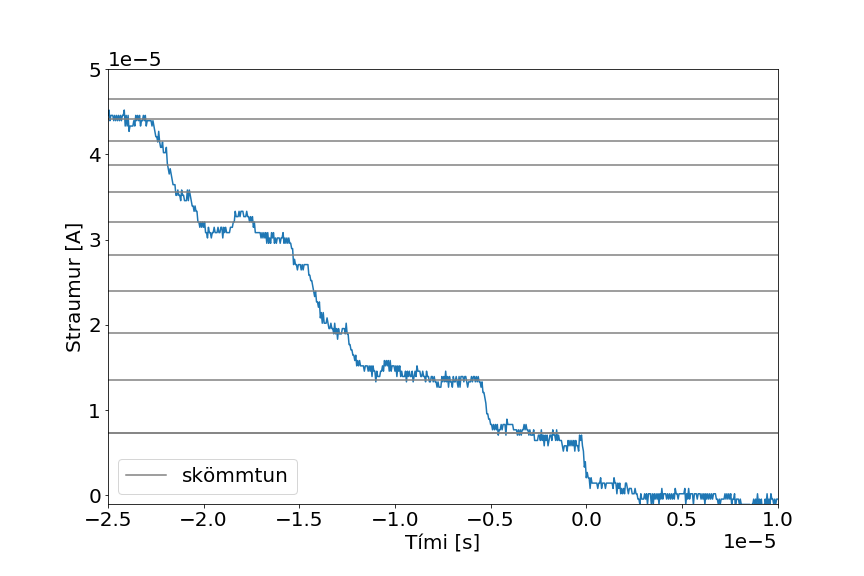
\includegraphics[width=0.8\textwidth]{kopar-straumur.png}
    \caption{Straumur í koparvírunum sem fall af tíma. Láréttu línurnar tákna skömmtuðu gildi straumsins sem búist er við miðað við líkanið.}
    \label{fig:kopar_straumur}
\end{figure}

Af mynd~\ref{fig:kopar_straumur} sést að við fáum, líkt og fyrir gullið, nokkuð skýr þrep í straummælingunni fyrir fyrstu nokkur skömmtunargildin, en þar fyrir ofan virðist straumurinn verða samfelldari. 

\begin{figure}[H]
    \centering
    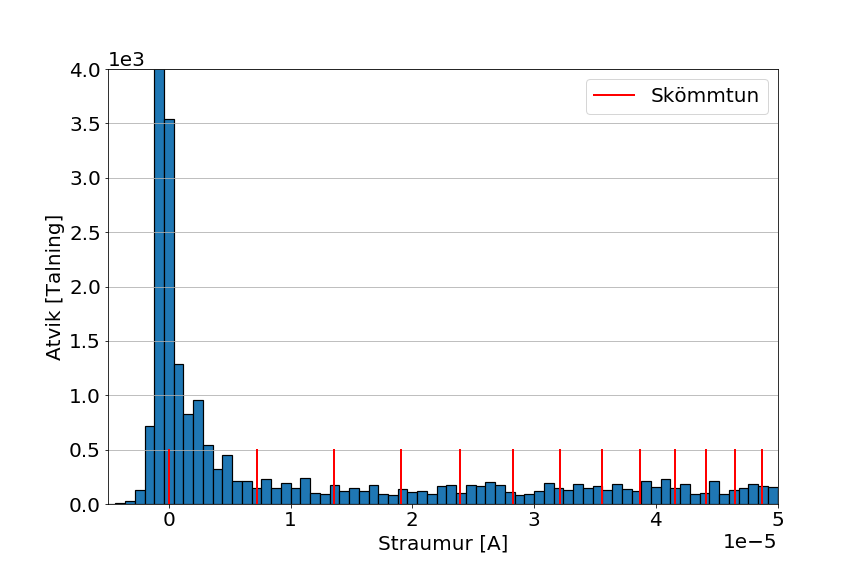
\includegraphics[width=0.8\textwidth]{kopar-hist-straumur.png}
    \caption{Tíðnirit fyrir mæld gildi straums í koparvírunum. Rauðu lóðréttu línurnar tákna skömmtuðu gildi straumsins sem búist er við miðað við líkanið.} 
    \label{fig:kopar_hist_straumur}
\end{figure}

Tíðniritið á mynd~\ref{fig:kopar_hist_straumur} sýnir örlitla toppa við fyrstu skömmtunargildin, en þaðan af er varla hægt að halda því fram að skömmtun sjáist. Gögnum er nú aftur breytt til þess að þau sýni leiðni.

\begin{figure}[H]
    \centering
    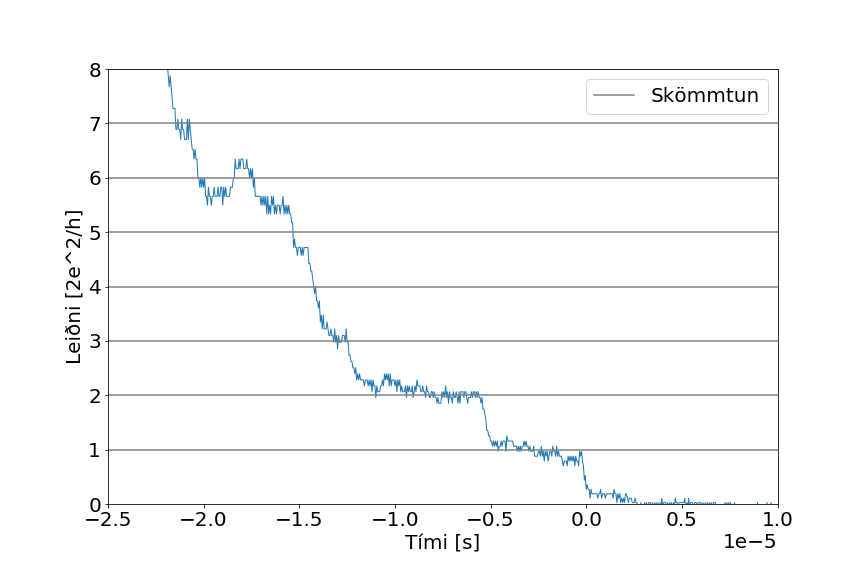
\includegraphics[width=0.8\textwidth]{kopar-leidni.png}
    \caption{Leiðni í koparvírunum sem fall af tíma. Láréttu línurnar tákna skömmtuðu gildi leiðninnar sem búist er við miðað við líkanið.}
    \label{fig:kopar_leidni}
\end{figure}

Eins og við var að búast er grafið fyrir leiðnina á mynd~\ref{fig:kopar_leidni} mjög sambærilegt grafinu fyrir straum á mynd~\ref{fig:kopar_straumur}.

\begin{figure}[H]
    \centering
    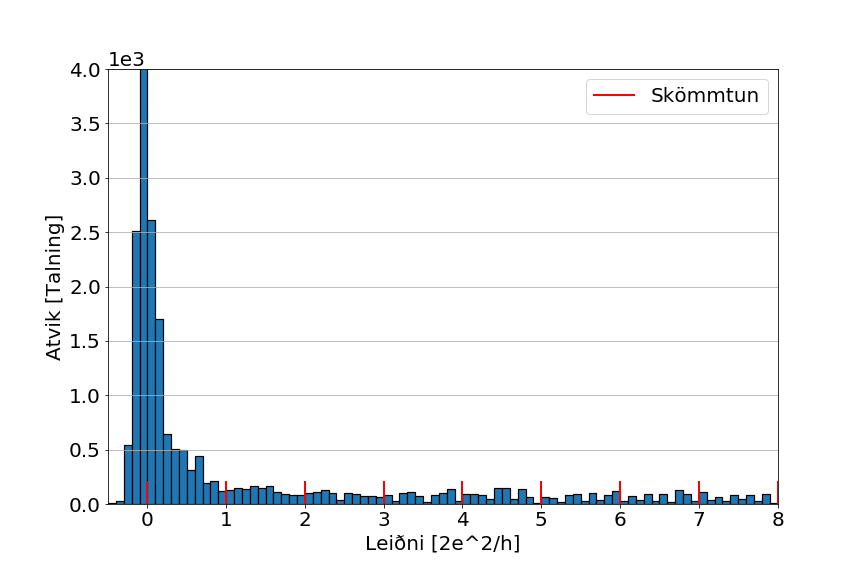
\includegraphics[width=0.8\textwidth]{kopar-hist-leidni.png}
    \caption{Tíðnirit fyrir mæld gildi leiðninnar í koparvírunum. Rauðu lóðréttu línurnar tákna skömmtuðu gildi sem búist er við miðað við líkanið.} 
    \label{fig:kopar_hist_leidni}
\end{figure}

Aftur fékkst aðeins lítill toppur fyrir fyrsta skömmtunargildið á mynd~\ref{fig:kopar_hist_leidni} en hæpið að tala um að hér sé mikil skömmtun fyrir $n > 1$.



\subsection{Platínu/Iridíum blanda}
%V_0 = 0.1025, 10% Ir, 250 micrometers
Síðasti vírinn sem var athugaður var $\SI{250}{\mu m}$ vír sem var $90\%$ platína ($\ce{Pt}$) og $10\%$ iridíum ($\ce{Ir}$). Straumurinn mældist aftur sem $\SI{0.1025}{V}$ og mælingar voru framkvæmdar á sama hátt og fyrr. Platína er mjög harður málmur þannig að ekki var við því búist að góðir nanóvírar myndu myndast. 

\begin{figure}[H]
    \centering
    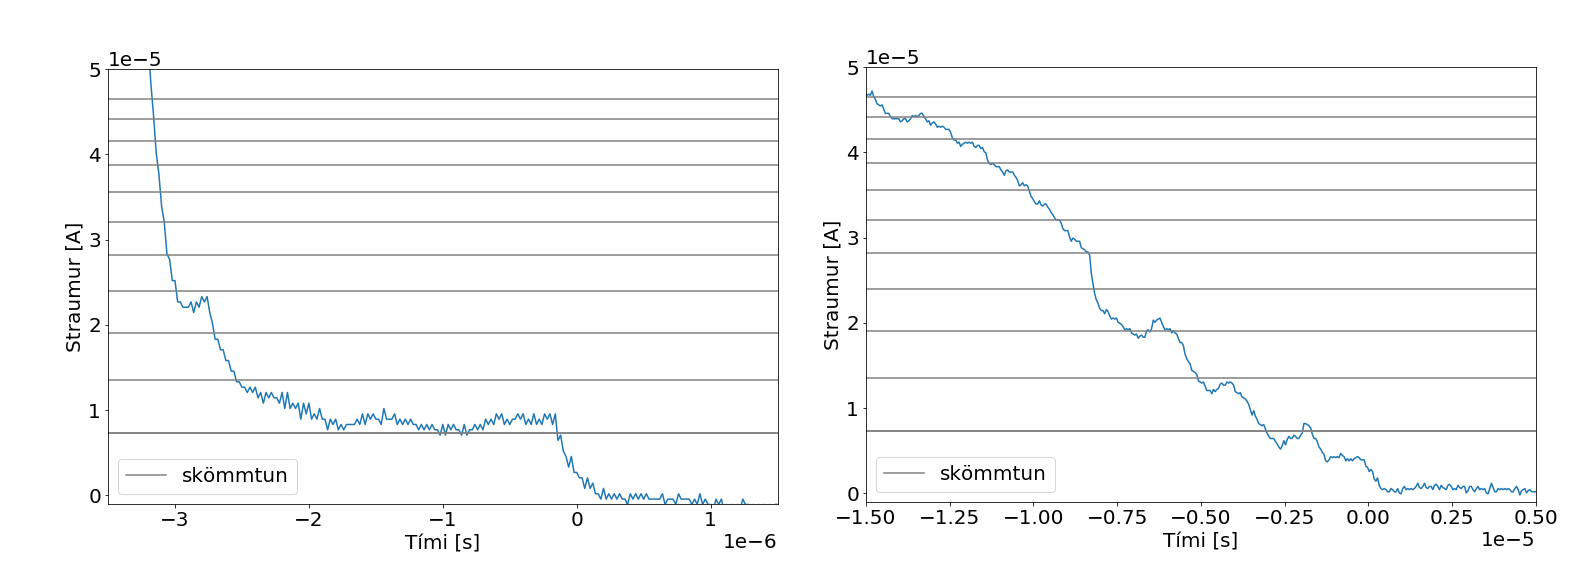
\includegraphics[width=1.0\textwidth]{saman-straumur.png}
    \caption{Straumur í $\ce{Pt}$-vírunum sem fall af tíma. Þessi gröf sýna þær tvær mælingar sem best virtust sýna skömmtun.}
    \label{fig:platina_straumur}
\end{figure}

Eins og sést hér á mynd~\ref{fig:platina_straumur} má greina einhverja örlitla skömmtun fyrir lægstu skömmtuðu gildin. Þrepin í straummælingunni voru þó langt frá því að vera jafn skýr og fyrir gull- og koparvírana.

\begin{figure}[H]
    \centering
    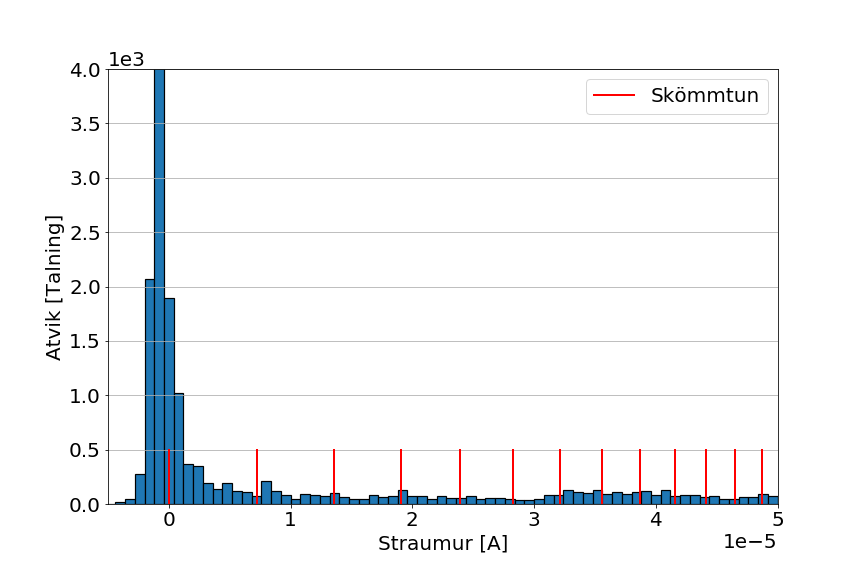
\includegraphics[width=0.8\textwidth]{plat-hist-straumur1.png}
    \caption{Tíðnirit fyrir mæld gildi straums í platínuvírunum. Rauðu lóðréttu línurnar tákna skömmtuðu gildi sem búist er við miðað við líkanið.}
    \label{fig:platina_hist_straumur}
\end{figure}

Við fáum nú nokkuð vel skilgreindan topp fyrir fyrsta skömmtunargildið, en þaðan af er ekki hægt að sjá að nein marktæk skömmtun finnist.


\begin{figure}[H]
    \centering
    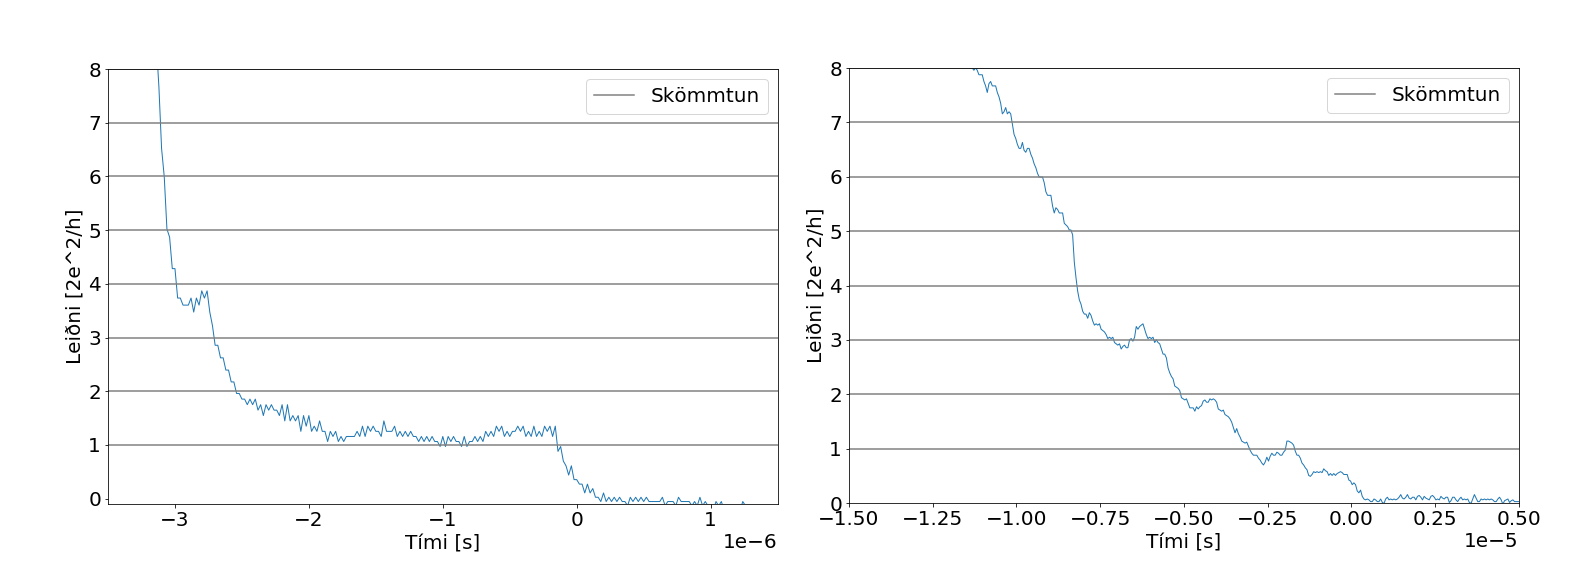
\includegraphics[width=1\textwidth]{saman-leidni.png}
    \caption{Leiðni í $\ce{Pt}$-vírunum sem fall af tíma. Þessi gröf sýna þær tvær mælingar sem best virtust sýna skömmtun.}
    \label{fig:platina_leidni}
\end{figure}

Líkt og áður virðast leiðnigröfin hér á mynd~\ref{fig:platina_leidni} mjög lík straumgröfunum á mynd~\ref{fig:platina_straumur}. Einhver vottur er hér af skömmtun en það er alls ekki mjög skýrt. 


\begin{figure}[H]
    \centering
    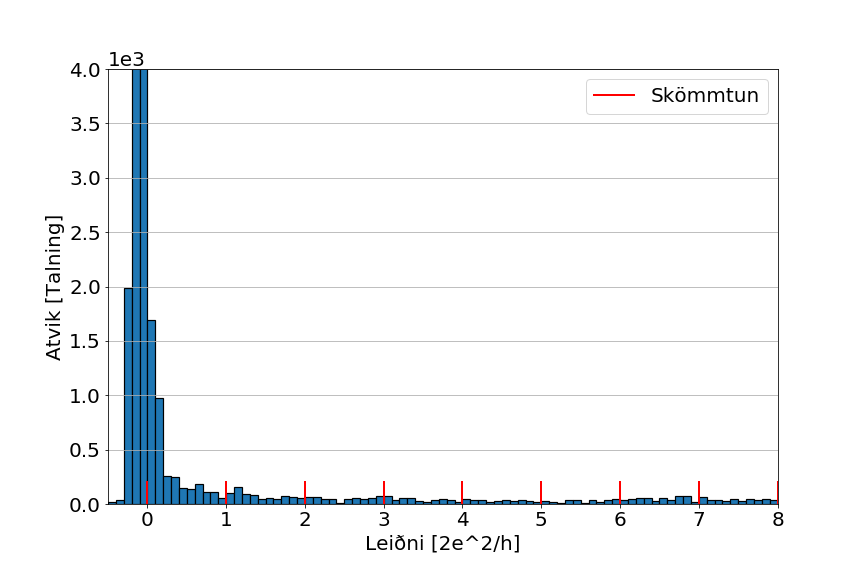
\includegraphics[width=0.8\textwidth]{plat-hist-leidni1.png}
    \caption{Tíðnirit fyrir mæld gildi leiðninnar í platínuvírunum. Rauðu lóðréttu línurnar tákna skömmtuðu gildi sem búist er við miðað við líkanið.}
    \label{fig:platina_hist_leidni}
\end{figure}

Hér á mynd~\ref{fig:platina_hist_leidni} sést, líkt og á mynd~\ref{fig:platina_hist_straumur}, að fyrsta skömmtunargildi leiðninnar mælist í einhverju magni, en þaðan af er nær enga skömmtun hægt að greina. 



\section{Samantekt}
Í öllum hlutum tilraunarinnar sjáum við áhrif skammtaleiðni koma fyrir en þau sjást misvel. Að okkar mati eru tíðniritin fyrir gullið (myndir \ref{fig:gull_hist_straumur} og \ref{fig:gull_hist_leidni}) að sýna skýrustu niðurstöðurnar en besta staka mælingin okkar er líklega sú sem við sýnum fyrir koparinn (mynd \ref{fig:kopar_straumur} og \ref{fig:kopar_leidni}). Tíðnirit kopars og platínu gefa ekki jafn góða niðurstöður og gullið gerir. Ástæða þess má líklega rekja til rangeygðra mælimanna en einnig er vert að nefna að tilraunin er erfið í framkvæmd og krefst mikillar þolinmæði. Dreifiliðurinn, $T$, gæti líka verið að hafa áhrif á mælingar okkar og er ólíklegt að sú nálgun að $T=1$ sé sönn.

\end{document}
